At this stage in the analysis, we are running low on simple cuts which can improve the signal-to-background ratio in the dataset. We must now turn to more complex solutions of separating the signal from potential background seepage. The first method we will use to do this is sPlot\cite{pivk_splot_2005}\footnote{This is stylized as ${}_s\mathcal{P}lot$ in the original paper, but I find this tedious to type and to read.}, a weighting scheme which corrects the na\"ive probabilistic weights one might first think to construct (dubbed ``inPlot'').

We start by developing a model for the signal and background probability distribution functions (PDFs) for a ``discriminating'' variable. We could then weight each event by some normalized probability of it being in the signal distribution rather than the background:

\begin{equation}
  w(x) = \frac{N_S f_S(x)}{N_S f_S(x) + N_B f_B(x)}
  \label{eq:splot:inplot-weights}
\end{equation}
where $x$ is the discriminating variable, $f_S(x)$ and $f_B(x)$ are the corresponding signal and background PDFs, and $N_S$ and $N_B$ are the total number of signal and background events, respectively.

However, as shown by Pivk and Le Diberder\cite{pivk_splot_2005}, we must be careful when using this procedure, as it will only correctly produce signal-isolated plots for ``control'' variables $y$ which are directly correlated with $x$. For the time being, let us assume that this is not the case, and that we wish to use the distribution of some variable which is uncorrelated with the variables we are plotting and analyzing\footnote{We will later see that things are not quite so simple!}. Following the sPlot derivation, we find that, to plot uncorrelated control variables, we must weight our data according to the following scheme:

\begin{equation}
  w(x) = \frac{V_{SS}f_S(x) + V_{SB}f_B(x)}{N_S f_S(x) + N_B f_B(x)},\quad \text{where } V^{-1}_{ij} = \sum_{x} \frac{f_i(x)f_j(x)}{\left(N_S f_S(x) + N_B f_B(x)\right)^2}
  \label{eq:splot:splot-weights}
\end{equation}

The $V^{-1}$ matrix can also be understood as the covariance matrix between the free parameters $N_S$ and $N_B$ in the fit of the signal-background mixture, $V^{-1}_{ij} = -N\pdv[2]{\ln\mathcal{L}}{N_i}{N_j}$, although there is reason to believe that direct calculation by this method will lead to less accurate results than the manual calculation in \Cref{eq:splot:splot-weights}\cite{dembinski_custom_2022}.

Now that we have a method of assigning weights, we must pick the discriminating variable. Typically, these weighting methods work well on the classic ``bump-on-a-background'' distributions, but because the mass of the kaons is constrained in the kinematic fit, the fitted mass of each kaon is just a $\delta$-function and combination of measured masses for each $\pi^+\pi^-$ pair will yield a Normal distribution with little to no apparent background (by construction), so we must be a bit more clever in determining a discriminating variable. By examining the BGGEN analysis done in {\color{red}[TODO: PREVIOUS SECTION]}, we can see that most likely sources of background arise when the intermediate kaons are missing from the reaction: $\gamma p \to 4\pi p$. This reaction shares the $K_SK_S$ final state exactly, so pairs of pions which look close enough to kaons will be almost indistinguishable in the data. However, they differ in one key way, namely that the $K_S$ intermediate contains a strange quark while the $\pi^+\pi^-$ decay state does not, so such a decay must occur via the weak interaction, which is notably slower than the strong interaction which would produce pion pairs with no intermediate kaon. In other words, while the signal's rest-frame lifetime distribution should have an exponential slope near the $K_S$ lifetime, the background would theoretically have nearly zero rest-frame lifetime for every event, or a much smaller exponential slope in practice.

Therefore, we will begin by generating both a signal and background dataset in Monte Carlo. We then interpret both datasets as if they were our desired channel by running them through the GlueX reconstruction and reaction filter, as well as all of our selections up to this point. We can then fit the rest-frame lifetime of each dataset to an exponential model,

\begin{equation}
  f(t; \lambda) = \lambda \exp{-\lambda t}
  \label{eq:splot:exponential}
\end{equation}
where $\lambda \equiv 1/\tau$, the lifetime of the kaon in question. Since we have two independently decaying kaons, we should really form a joint distribution for both, where we will assume each kaon has the same average lifetime:
\begin{equation}
  f(t_1, t_2; \lambda) = \lambda^2 \exp{-\lambda t_1}\exp{-\lambda t_2}
  \label{eq:splot:exponential_joint}
\end{equation}
Both the signal and background distributions can be modeled in this way, giving us only two free parameters, $\lambda_S$ and $\lambda_B$ for the signal and background respectively, to fit.


Once we obtain nominal values for $\lambda_S$ and $\lambda_B$ from fits over the signal and background Monte Carlo, we can fix the exponential slopes to the fit values and perform a new fit to our real data with a mixture model:
\begin{align}
  g(t_1, t_2) &\equiv z f(t_1, t_2; \lambda)\eval_{\lambda=\lambda_S} + (1-z) f(t_1, t_2; \lambda)\eval_{\lambda=\lambda_B} \notag\\
              &= z \lambda_S^2\exp{-\lambda_S t_1}\exp{-\lambda_S t_2} + (1-z) \lambda_B^2\exp{-\lambda_B t_1}\exp{-\lambda_B t_2}
  \label{eq:splot:mixture}
\end{align}

In the fit to data, only the fraction of signal to background, $z$, is floating. From its fit value, we can determine values of $N_S$ and $N_B$ to use in \Cref{eq:splot:splot_weights} and complete the weighting procedure.

\subsection{Non-Factorizing sPlot}\label{sec:non-factorizing-splot}

Over the course of the previous discussion, it was assumed that the discriminating variable, $t$, was statistically independent from the control variable. To test whether this is indeed true, we need to first pick some control variables which we want to be able to use later. The set of control variables must include all variables we use as inputs to the partial-wave analysis in \Cref{ch:partial-wave-analysis}. This includes the invariant mass $m$ of the $K_S^0K_S^0$ system and the helicity angles $\theta$ and $\varphi$ of the decay. To test for independence, we first split our dataset into $M$ evenly-spaced quantiles in the control variable, which ensures each bin gets roughly the same number of events. Next, we calculate the likelihood of the null hypothesis, which assumes the variables are statistically independent, by fitting all datasets simultaneously with a shared $\lambda$ parameter. We then calculate the likelihood of the alternative hypothesis, which assumes statistical dependence, by finding the joint likelihood of independent fits of $\lambda$ over each quantile. The result of these fits can be formulated as a likelihood ratio,

\begin{equation}
  \Lambda = -2\ln\frac{\sup \mathcal{L}_{H_0}}{\sup \mathcal{L}_{H_1}} = -2\ln\frac{\sup \prod_i^M \mathcal{L}_i(z_i, \lambda_S, \lambda_B)}{\sup \prod_i^M \mathcal{L}_i(z_i, \lambda_{S,i}, \lambda_{B,i})}
  \label{eq:independence-test}
\end{equation}

$\Lambda$ is $\chi^2$ distributed with $2M - 2$ degrees of freedom (the difference between $M + 2$ free parameters in the null hypothesis and $3M$ in the alternative hypothesis). Note that here, $\mathcal{L}_i$ denotes the likelihood evaluated over data in the $i$th quantile. The factor of $2$ is required because $\ln\mathcal{L}(\theta_1,...,\theta_i) \sim -\frac{1}{2}\chi^2_i$ asymptotically with sample size according to Wilks' theorem. We can obtain a $p$-value representing the likelihood of the null hypothesis being true by evaluating the $p$-value:

\begin{equation}
  p = 1 - F_{\chi^2_{2M-2}}(\Lambda) = 1 - P\left(\frac{2M-2}{2}, \frac{\Lambda}{2}\right)
  \label{eq:significance-test}
\end{equation}}

where $P(s, t)$ is the regularized gamma function. Following this procedure for the invariant mass of $K_S^0K_S^0$\footnote{No significant statistical dependence was found for the helicity angles.}, the $p$-values for each number of quantiles and run period can be seen in the first four rows of \Cref{tab:factorization-results} and in \Cref{fig:data-factorization-fit}, depicting the case with four quantiles. The calculated $p$-values tend to be very small, implying that we should reject the null hypothesis and accept that the discriminating (rest-frame lifetime) and control (invariant mass of $K_S^0K_S^0$) variables are not statistically independent. This means we cannot use a traditional sPlot to weight our data. Fortunately, the process for obtaining the correct weights is straightforward, we simply allow for more than one signal and background component in the fit and sum over all signal components when we calculate the final weight values~\cite{dembinski_custom_2022}. Since sPlot weights from different components can be added to each other to obtain a joint weight~\cite{pivk_splot_2005}, \Cref{eq:splot:splot-weights} can be extended to multiple signal and background components:

\begin{equation}
  w_{\mathbb{S}}(x) = \frac{\sum_{i\in\mathbb{S}}\sum_{j} V_{ij}f_j(x)}{\sum_{k}N_kf_k(x)},\quad \text{where } V_{ij}^{-1} = \sum_{x} \frac{f_i(x)f_j(x)}{\left(\sum_{k} N_kf_k(x)\right)^2}
  \label{eq:splot:splot-weights-factorizing}
\end{equation}

and $\mathbb{S}$ is the set of signal components. We can further verify the need for non-factorizing sPlot by performing the factorization test described in \Cref{eq:independence-test,eq:significance-test} to the signal and background Monte Carlo, with a slight modification to the number of free parameters, since we only need to fit either a signal or background component rather than a mixture:

\begin{equation}
  p = 1 - P\left(\frac{M-1}{2}, \frac{\Lambda}{2}\right) \quad\text{where }\Lambda = -2\ln\frac{\sup\prod_i^M \mathcal{L}_i(\lambda)}{\sup\prod_i^M \mathcal{L}_i(\lambda_i)}
  \label{eq:independence-test-mc}
\end{equation}

The results of these tests can also be found in the last eight rows of \Cref{tab:factorization-results}, and are visualized for four quantiles in \Cref{fig:mc-factorization-fits}. There are enough significantly small $p$-values to justify the use of non-factorizing sPlot across both the signal and background components, meaning that we need at least two signal and two background components in the final sPlot weighting.

\begin{table}
  \begin{center}
    \begin{tabular}{ccccc}\toprule
       & & \multicolumn{3}{c}{\# quantiles} \\\cmidrule(lr){3-5}
       & & 2 & 3 & 4 \\
       Data Type & Run Period & $p$ & $p$ & $p$ \\\midrule
      Data & Spring 2017 & $1.36 \times 10^{-28}$ & $1.92 \times 10^{-27}$ & $8.00 \times 10^{-29}$\\
       & Spring 2018 & $3.38 \times 10^{-08}$ & $1.32 \times 10^{-07}$ & $6.09 \times 10^{-09}$\\
       & Fall 2018 & $2.18 \times 10^{-09}$ & $5.44 \times 10^{-15}$ & $1.02 \times 10^{-15}$\\
       & Spring 2020 & $9.86 \times 10^{-171}$ & $2.10 \times 10^{-199}$ & $1.08 \times 10^{-198}$\\\midrule
      $K_S^0K_S^0$ MC & Spring 2017 & $<2.23\times 10^{-308}$ & $<2.23\times 10^{-308}$ & $<2.23\times 10^{-308}$\\
       & Spring 2018 & $<2.23\times 10^{-308}$ & $<2.23\times 10^{-308}$ & $<2.23\times 10^{-308}$\\
       & Fall 2018 & $<2.23\times 10^{-308}$ & $<2.23\times 10^{-308}$ & $<2.23\times 10^{-308}$\\
       & Spring 2020 & $<2.23\times 10^{-308}$ & $<2.23\times 10^{-308}$ & $<2.23\times 10^{-308}$\\\midrule
      $4\pi$ MC & Spring 2017 & $9.53 \times 10^{-01}$ & $4.78 \times 10^{-03}$ & $5.62 \times 10^{-02}$\\
       & Spring 2018 & $6.40 \times 10^{-01}$ & $9.78 \times 10^{-01}$ & $4.49 \times 10^{-01}$\\
       & Fall 2018 & $1.54 \times 10^{-05}$ & $1.44 \times 10^{-06}$ & $6.46 \times 10^{-07}$\\
       & Spring 2020 & $4.47 \times 10^{-09}$ & $2.36 \times 10^{-08}$ & $2.25 \times 10^{-09}$\\\bottomrule
    \end{tabular}
    \caption{The probability of accepting the null hypothesis (that the rest-frame lifetime is statistically independent of the invariant mass of $K_S^0K_S^0$) for the tests described in \Cref{eq:independence-test} for data and \Cref{eq:independence-test-mc} for Monte Carlo with the given number of quantiles. All values are calculated with a $\chi^2_\nu < 3.0$ selection on each type of data over each run period. Values listed as $<2.23 \times 10^{-308}$ are nonzero but smaller than the smallest representable 64-bit floating point number}\label{tab:factorization-results}
  \end{center}
\end{table}

\begin{figure}
  \begin{center}
    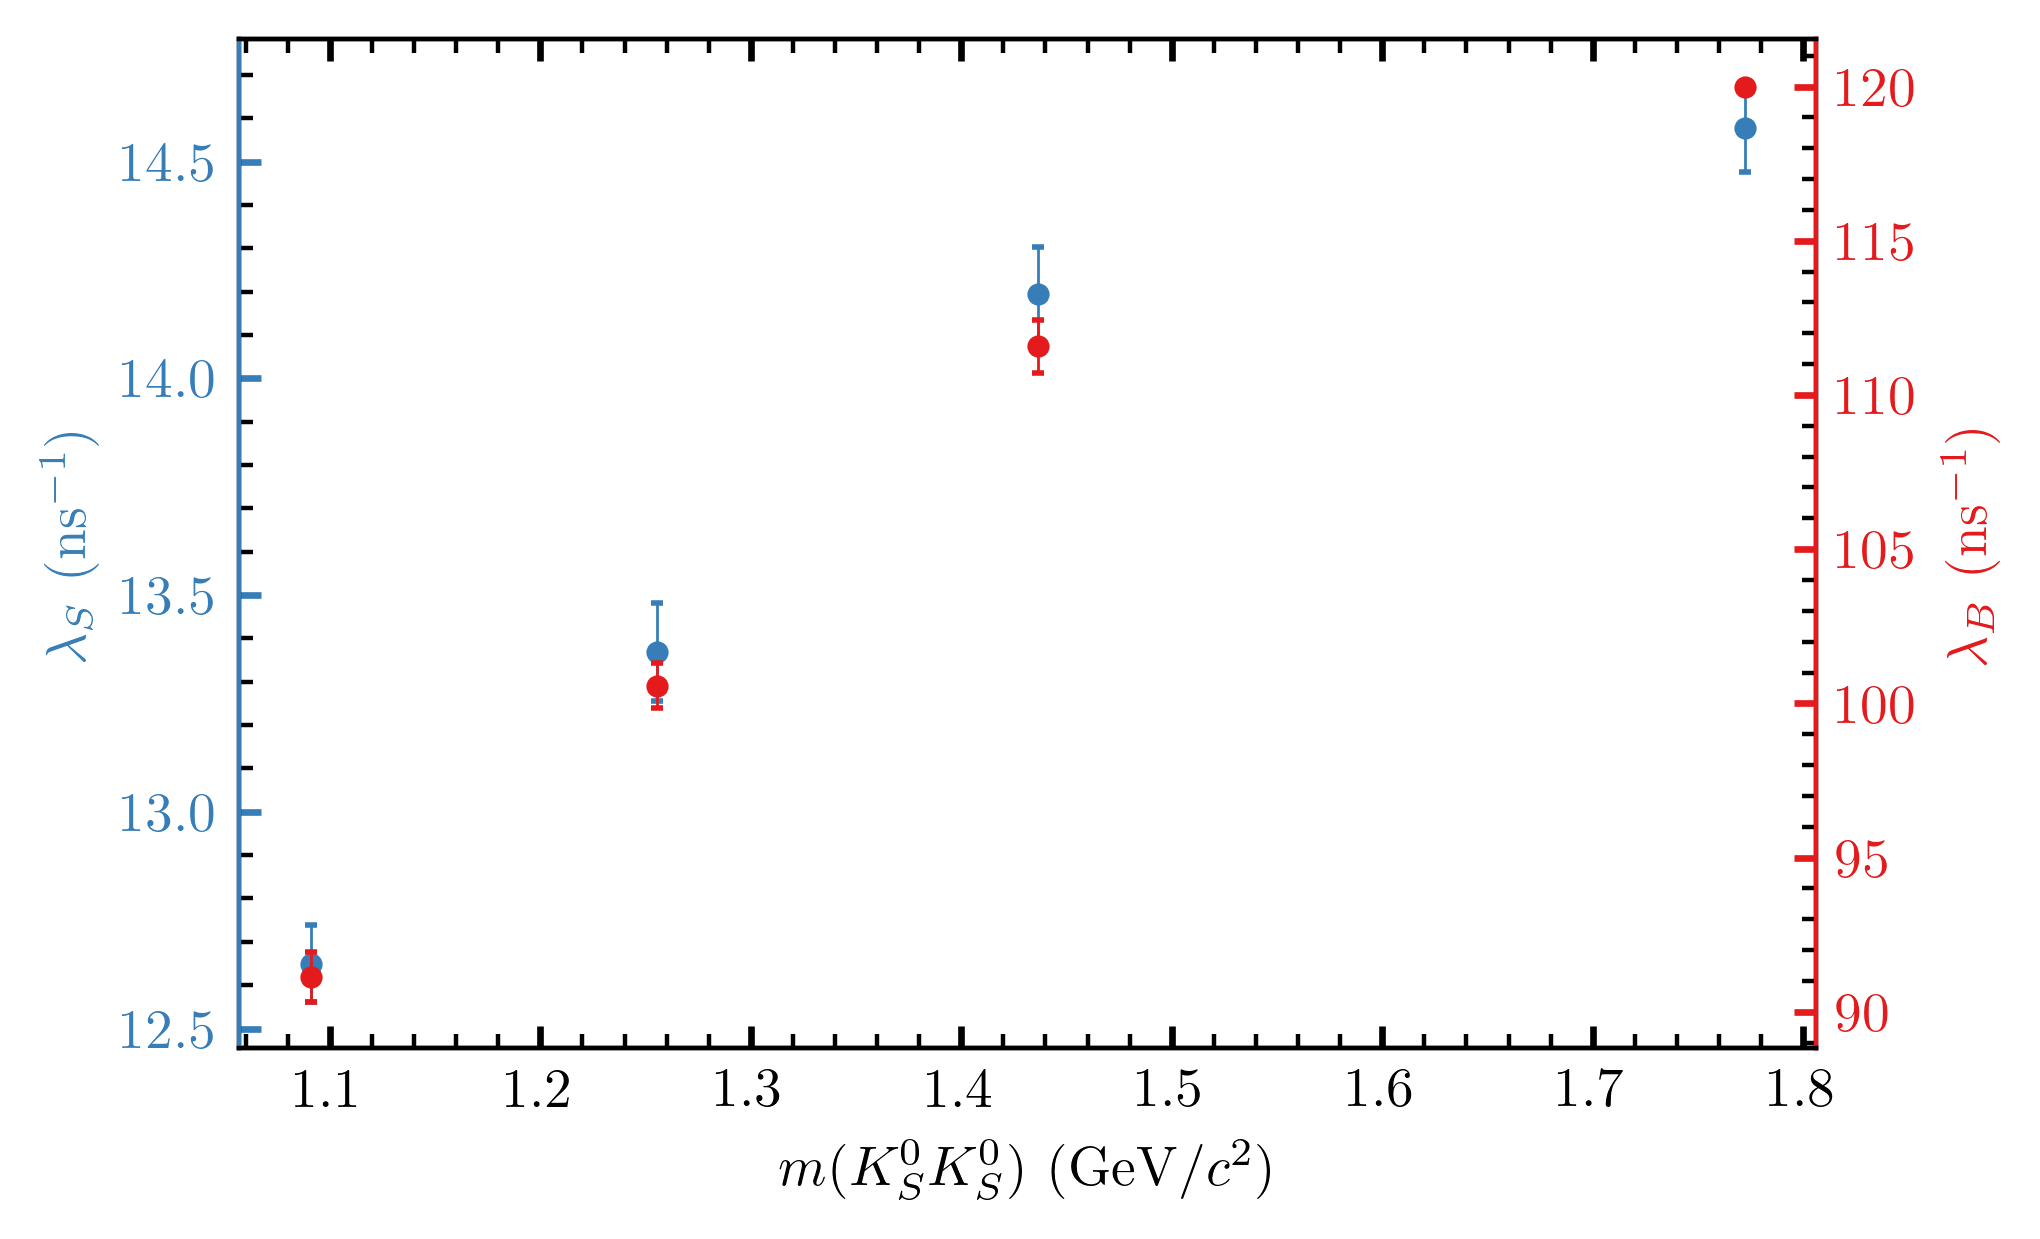
\includegraphics[width=.8\columnwidth]{factorization_plot_data_s20_chisqdof_3.0_4_quantiles.png}
  \end{center}
  \caption{Exponential slopes from fits over four quantiles in $m(K_S^0K_S^0)$ ($x$-axis) to a mixture of signal (left $y$-axis) and background (right $y$-axis) components for the Spring 2020 run period. These fits show a definite statistical dependence between rest-frame lifetime and the invariant mass of $K_S^0K_S^0$, as described in \Cref{tab:factorization-results}. All values are calculated with a $\chi^2_\nu < 3.0$ selection on each type of data over each run period.}\label{fig:data-factorization-fit}
\end{figure}

\begin{figure}
  \begin{center}
    \begin{subfigure}[b]{.8\columnwidth}
      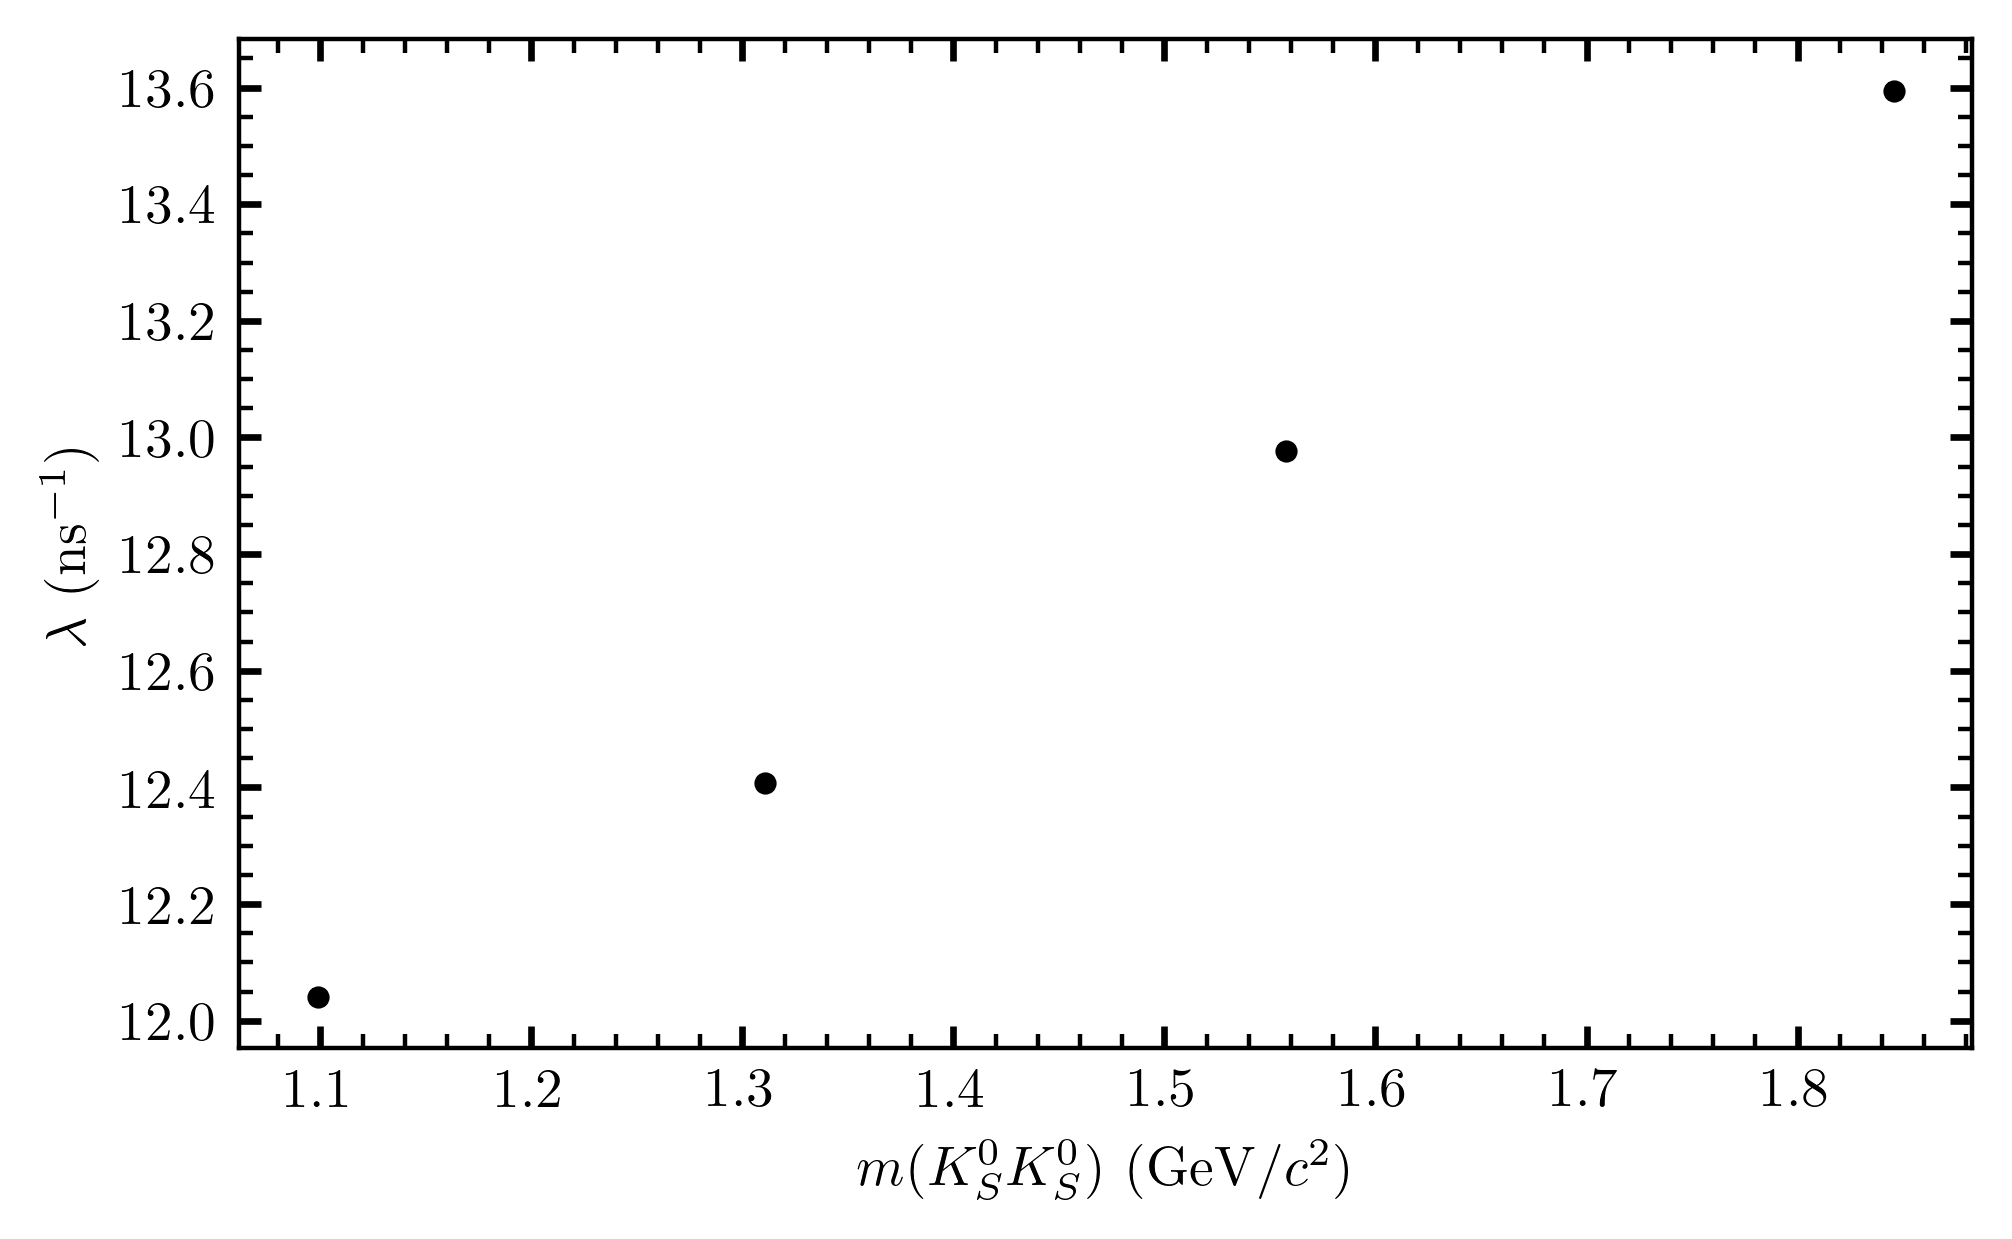
\includegraphics[width=1\linewidth]{factorization_plot_accmc_s20_chisqdof_3.0_4_quantiles.png}
      \caption{}
      \label{fig:mc-factorization-fits-a}
    \end{subfigure}
    \begin{subfigure}[b]{.8\columnwidth}
      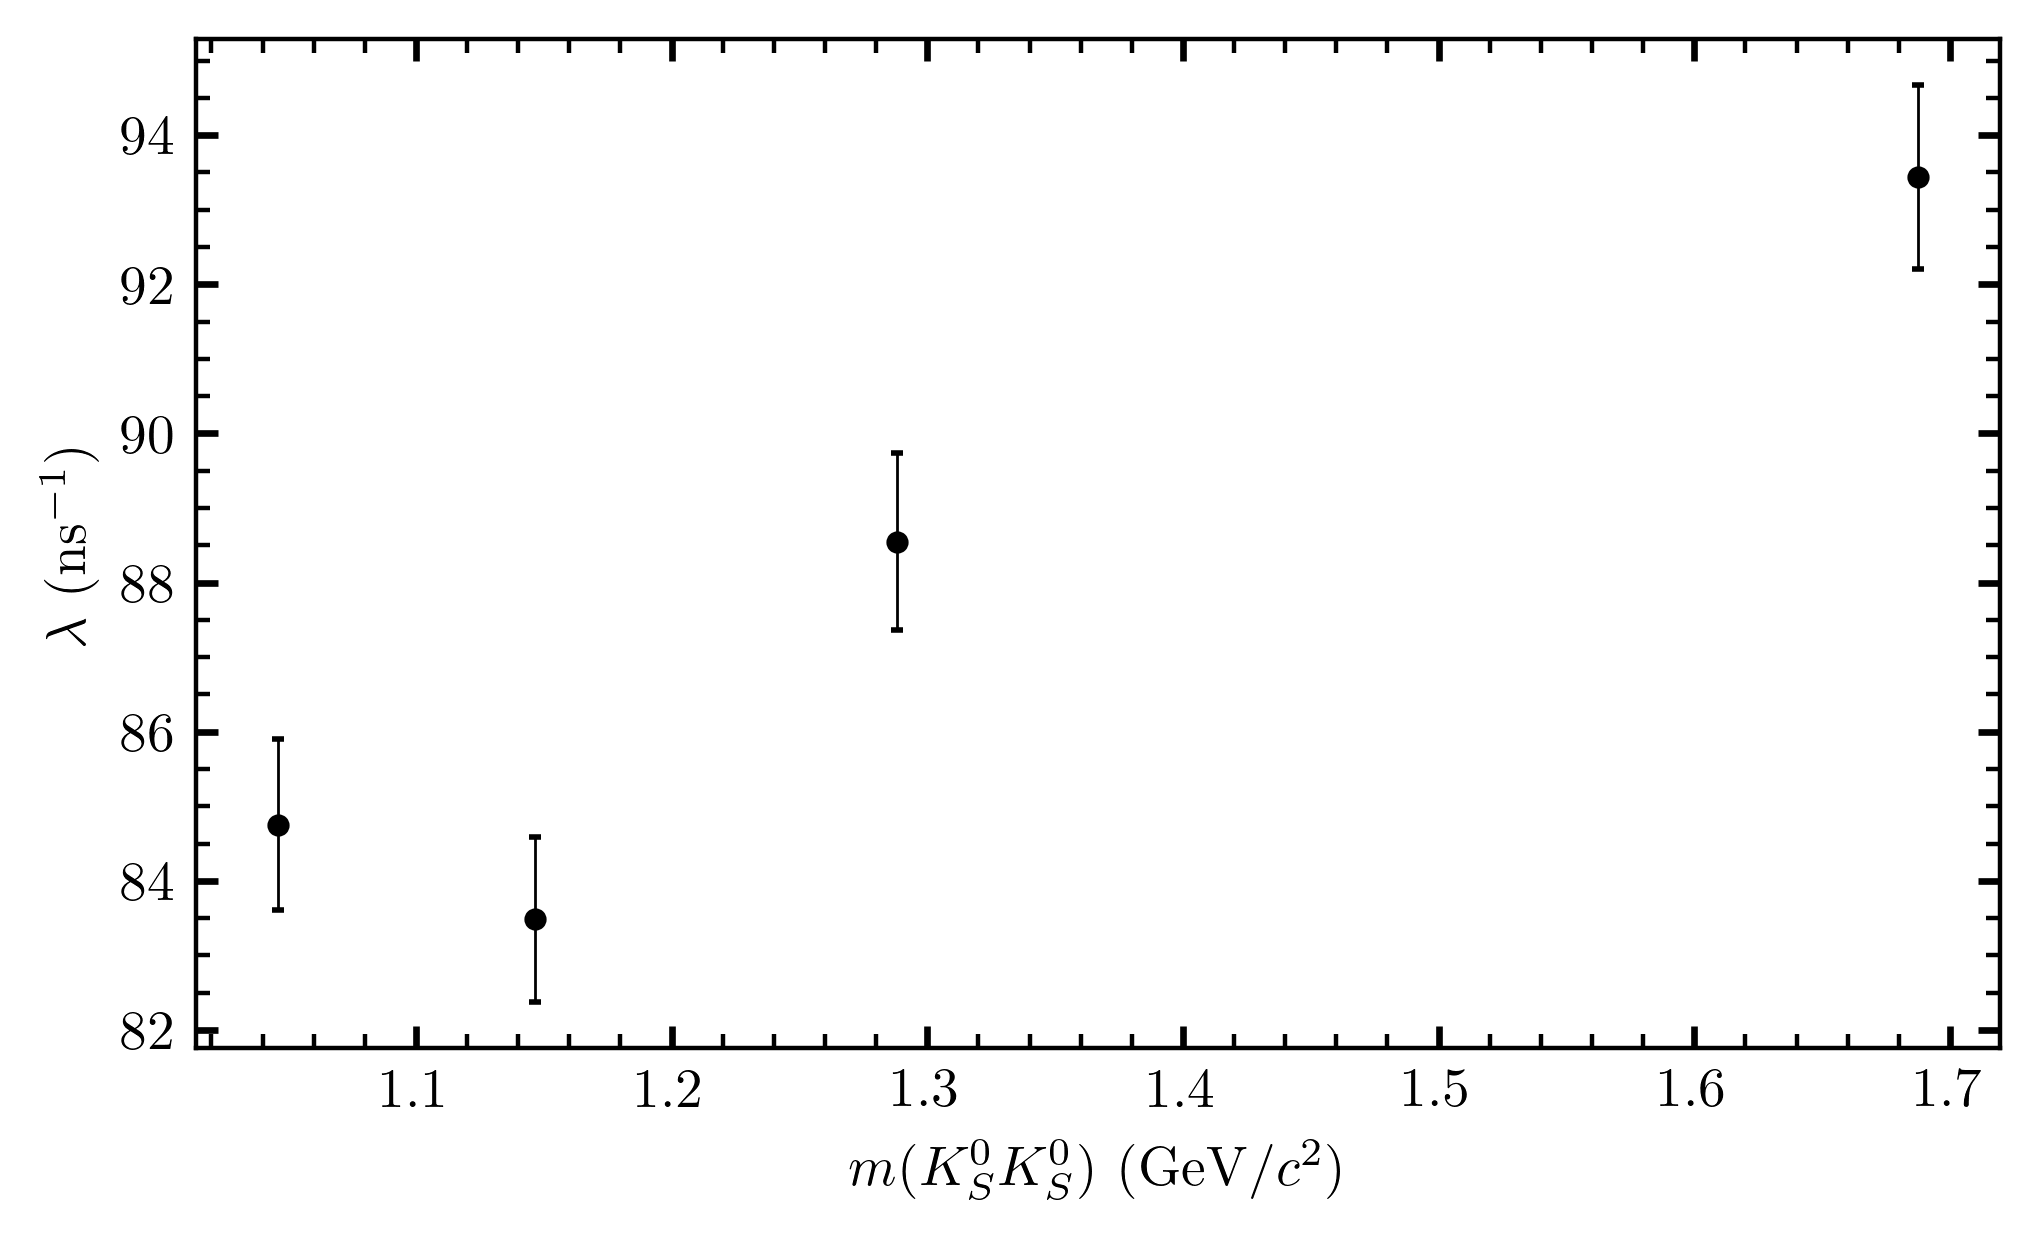
\includegraphics[width=1\linewidth]{factorization_plot_bkgmc_s20_chisqdof_3.0_4_quantiles.png}
      \caption{}
      \label{fig:mc-factorization-fits-b}
    \end{subfigure}
  \end{center}
  \caption{Exponential slopes from fits over four quantiles in $m(K_S^0K_S^0)$ ($x$-axis) of the signal (a) and background (b) Monte Carlo rest-frame lifetime distributions for the Spring 2020 run period. Both show a definite statistical dependence between rest-frame lifetime and the invariant mass of $K_S^0K_S^0$, as described in \Cref{tab:factorization-results}. All values are calculated with a $\chi^2_\nu < 3.0$ selection on each type of data over each run period.}\label{fig:mc-factorization-fits}
\end{figure}

\subsection{Application of Weights}\label{sec:application-of-weights}

The only thing left to do is determine how many signal and background components we should use in the weighting procedure. To this end, we now turn to the Monte Carlo simulations of the signal and $4\pi$-background. By choosing a number of quantiles in invariant mass corresponding to the number of components, we can fit single exponential distributions to each quantile in the simulated signal and background. For instance, if we chose to use two signal components and three background components, we would divide the signal Monte Carlo into two quantiles and the background Monte Carlo into three, and fit each quantile to an exponential distribution to obtain a set of two $\lambda_S$ and three $\lambda_B$ values. The resulting $\lambda_S$ and $\lambda_B$ values could then be used as a starting point for a multi-component fit to the data. Alternatively, both the signal and background or just the signal could be fixed to the values from the fits to simulations, and only the yields (or the yields and background $\lambda$s) would be allowed to float in the fit to data. We will refer to the first case, where the fit parameters from Monte Carlo are free, as $A$, the case where the signal $\lambda$s are fixed as $B$, and the case where all $\lambda$s are fixed (and the only floating parameters are the yields of each component) as $C$. To select a model, we can use the relative Akaike Information Criterion (AIC)~\cite{akaike_information_1998} and Bayesian Information Criterion (BIC)~\cite{schwarz_estimating_1978}:
\begin{alignat}{2}
  r\text{AIC} &\equiv \text{AIC} - \text{AIC}_\text{min} \quad\text{where } \text{AIC} &&\equiv 2k - 2\ln\mathcal{L} \\
  r\text{BIC} &\equiv \text{BIC} - \text{BIC}_\text{min} \quad\text{where } \text{BIC} &&\equiv k\ln{N} - 2\ln\mathcal{L} \\
  \label{eq:information-criteria}
\end{alignat}
where $k$ is the number of free parameters and $N$ is the number of events in the dataset. The optimal model will minimize these criteria. In \Cref{tab:factorization-results}, all of the relative AIC and BIC values are shown. Excluding cases with only one signal or background component (restricting to models which have non-factorizing signal and background components), the minimizing values for most run periods tend to use two signal and two background components, and excluding the Spring 2020 dataset, they all use method $B$, where the signal components are fixed to values obtained from Monte Carlo while the background components are initialized at Monte Carlo values but allowed to float in the fit. For consistency, we will use method $B$ with two signal and two background components, denoted $B(2,2)$, as our weighting method. See \Cref{fig:splot-data-fit}. The selection of method $B$ is also interesting as it could describe a case where another background which is not modeled in the background Monte Carlo is present and has a similar exponential slope. Since these slopes are free in the fit to the data, they may anticipate this unknown slope better than the fixed case (method $C$), and method $B$ also explicitly assumes the Monte Carlo for true signal kaons is correct and fixes their component slopes (unlike method $A$).

\begin{table}
  \begin{center}
    \begin{tabular}{ccccccccccccc}\toprule
    & \multicolumn{2}{c}{\# Components} & \multicolumn{2}{c}{Spring 2017} & \multicolumn{2}{c}{Spring 2018} & \multicolumn{2}{c}{Fall 2018} & \multicolumn{2}{c}{Spring 2020}\\\cmidrule(lr){2-3}\cmidrule(lr){4-5}\cmidrule(lr){6-7}\cmidrule(lr){8-9}\cmidrule(lr){10-11}
      Method & Signal & Background & $r\text{AIC}$ & $r\text{BIC}$ & $r\text{AIC}$ & $r\text{BIC}$ & $r\text{AIC}$ & $r\text{BIC}$ & $r\text{AIC}$ & $r\text{BIC}$\\\midrule
      $A$ & $1$ & $1$ & \underline{$0.000$} & \underline{$0.000$} & \underline{$0.000$} & \underline{$0.000$} & \underline{$0.000$} & \underline{$0.000$} & $51.876$ & $8.573$\\
       & $1$ & $2$ & $4.000$ & $21.835$ & $4.000$ & $23.028$ & $4.000$ & $23.490$ & $32.397$ & $10.746$\\
       & $1$ & $3$ & $8.000$ & $43.668$ & $8.002$ & $46.059$ & $8.005$ & $46.985$ & $36.827$ & $36.827$\\
       & $2$ & $1$ & $4.000$ & $21.834$ & $4.000$ & $23.028$ & $4.000$ & $23.490$ & $46.866$ & $25.215$\\
       & $2$ & $2$ & $8.000$ & $43.669$ & $8.004$ & $46.061$ & $8.000$ & $46.980$ & \fcolorbox{red}{white}{\underline{$0.000$}} & \fcolorbox{red}{white}{\underline{$0.000$}}\\
       & $2$ & $3$ & $12.000$ & $65.503$ & $12.001$ & $69.086$ & $12.004$ & $70.473$ & $54.865$ & $76.516$\\
       & $3$ & $1$ & $8.000$ & $43.669$ & $8.000$ & $46.057$ & $8.000$ & $46.980$ & $31.906$ & $31.906$\\
       & $3$ & $2$ & $12.000$ & $65.503$ & $12.002$ & $69.087$ & $12.001$ & $70.470$ & $54.357$ & $76.008$\\
       & $3$ & $3$ & $16.001$ & $87.338$ & $16.000$ & $92.114$ & $16.003$ & $93.962$ & $0.897$ & $44.200$\\\midrule
      $B$ & $1$ & $1$ & $51.318$ & $42.400$ & $46.523$ & $37.008$ & $78.990$ & $69.245$ & $435.265$ & $381.136$\\
       & $1$ & $2$ & $47.778$ & $56.695$ & $50.523$ & $60.037$ & $69.623$ & $79.368$ & $215.025$ & $182.548$\\
       & $1$ & $3$ & $51.126$ & $77.878$ & $54.524$ & $83.066$ & $72.976$ & $102.210$ & $222.971$ & $212.146$\\
       & $2$ & $1$ & $7.891$ & $7.891$ & $0.635$ & $0.635$ & $1.056$ & $1.056$ & $129.068$ & $85.765$\\
       & $2$ & $2$ & $11.891$ & \fcolorbox{red}{white}{$29.725$} & \fcolorbox{red}{white}{$4.635$} & \fcolorbox{red}{white}{$23.663$} & \fcolorbox{red}{white}{$5.057$} & \fcolorbox{red}{white}{$24.547$} & $52.986$ & $31.334$\\
       & $2$ & $3$ & $15.893$ & $51.561$ & $8.635$ & $46.692$ & $9.059$ & $48.038$ & $58.202$ & $58.202$\\
       & $3$ & $1$ & $2.496$ & $11.413$ & $3.770$ & $13.284$ & $2.411$ & $12.156$ & $75.783$ & $43.306$\\
       & $3$ & $2$ & \fcolorbox{red}{white}{$6.498$} & $33.250$ & $7.770$ & $36.313$ & $6.422$ & $35.657$ & $35.672$ & $24.846$\\
       & $3$ & $3$ & $10.496$ & $55.082$ & $11.770$ & $59.341$ & $10.411$ & $59.135$ & $40.264$ & $51.090$\\\midrule
      $C$ & $1$ & $1$ & $215.228$ & $197.394$ & $639.813$ & $620.785$ & $695.587$ & $676.098$ & $2698.867$ & $2633.913$\\
       & $1$ & $2$ & $216.138$ & $207.221$ & $610.406$ & $600.892$ & $461.384$ & $451.640$ & $1822.845$ & $1768.716$\\
       & $1$ & $3$ & $169.934$ & $169.934$ & $624.358$ & $624.358$ & $352.522$ & $352.522$ & $1521.662$ & $1478.359$\\
       & $2$ & $1$ & $205.960$ & $197.043$ & $649.757$ & $640.242$ & $697.047$ & $687.302$ & $2695.194$ & $2641.066$\\
       & $2$ & $2$ & $206.778$ & $206.778$ & $619.947$ & $619.947$ & $453.115$ & $453.115$ & $1778.976$ & $1735.673$\\
       & $2$ & $3$ & $155.836$ & $164.754$ & $634.060$ & $643.574$ & $337.024$ & $346.769$ & $1455.471$ & $1422.994$\\
       & $3$ & $1$ & $209.102$ & $209.102$ & $645.091$ & $645.091$ & $695.880$ & $695.880$ & $2692.864$ & $2649.561$\\
       & $3$ & $2$ & $209.927$ & $218.844$ & $615.616$ & $625.130$ & $453.630$ & $463.375$ & $1781.688$ & $1749.211$\\
       & $3$ & $3$ & $159.336$ & $177.171$ & $629.602$ & $648.630$ & $338.314$ & $357.803$ & $1459.431$ & $1437.780$\\\bottomrule
    \end{tabular}
    \caption{Relative AIC and BIC values for each fitting method (relative within each run period). The absolute minimum values in each column are underlined, and the minimums excluding models with only one signal or background component are boxed.}\label{tab:splot-model-results}
  \end{center}
\end{table}

\begin{figure}
  \begin{center}
    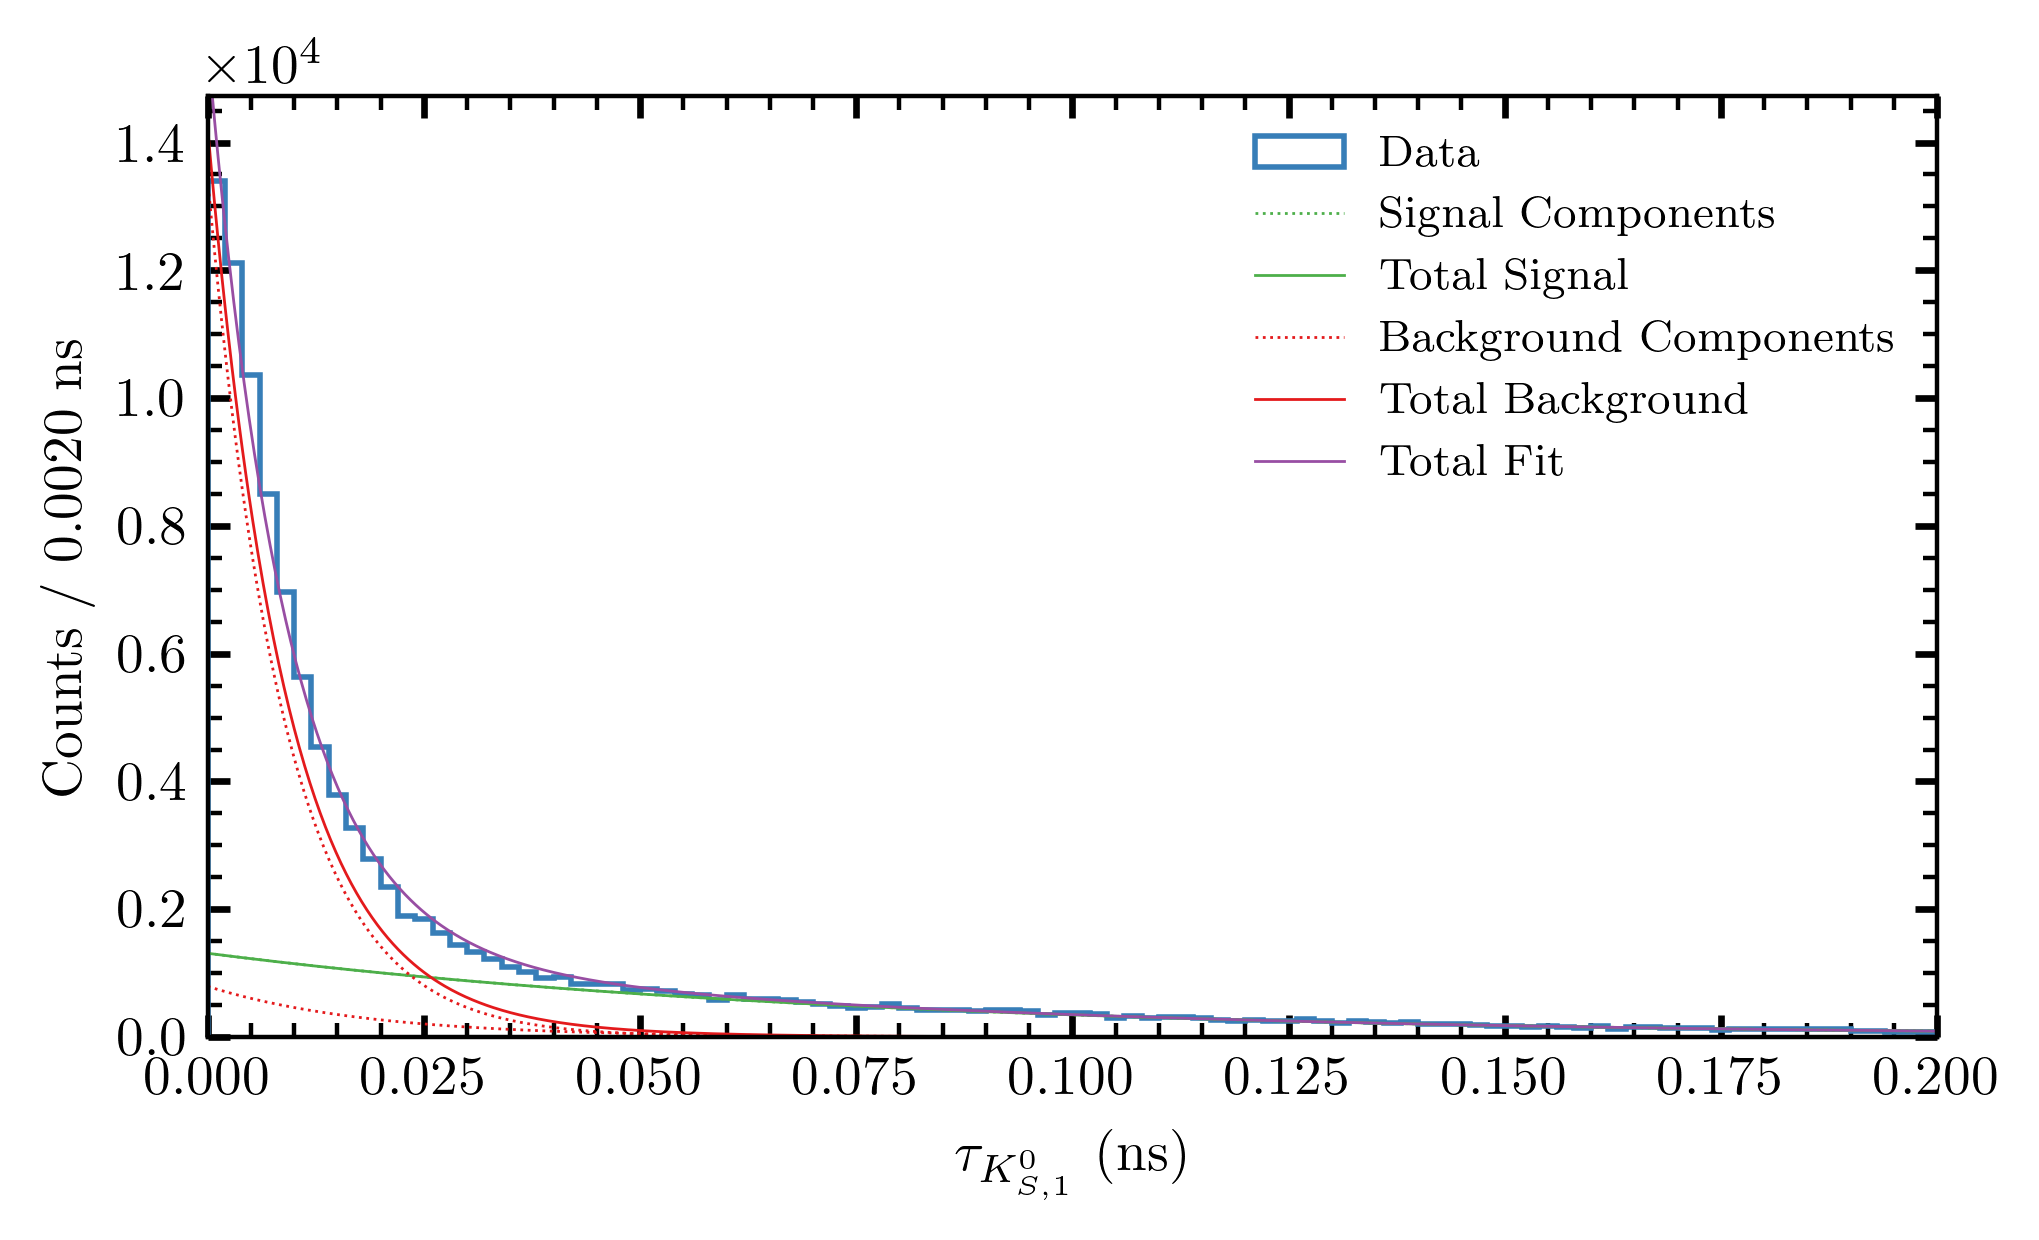
\includegraphics[width=.8\columnwidth]{splot_fit_data_s20_chisqdof_3.0_splot_B_2s_2b.png}
  \end{center}
  \caption{Fit of \Cref{eq:splot:mixture} to data from the Spring 2020 run period using method $B(2,2)$. True kaon events are prominent in the tail of the distribution, whereas background events peak strongly near zero. All values are calculated with a $\chi^2_\nu < 3.0$ selection on each type of data over each run period. The second signal component tends to be very small but non-zero across all datasets.}\label{fig:splot-data-fit}
\end{figure}

